% !TEX root = ../../main.tex
\section{Artificial Data}\label{sec:artificial_data}
\TODO{Use data from \cite{camci2010change,takeuchi2006unifying}}
In this section we present three data sets as used by \cite{camci2010change,takeuchi2006unifying} to provide for a objetive performance comparison.

\begin{figure}
\centering
  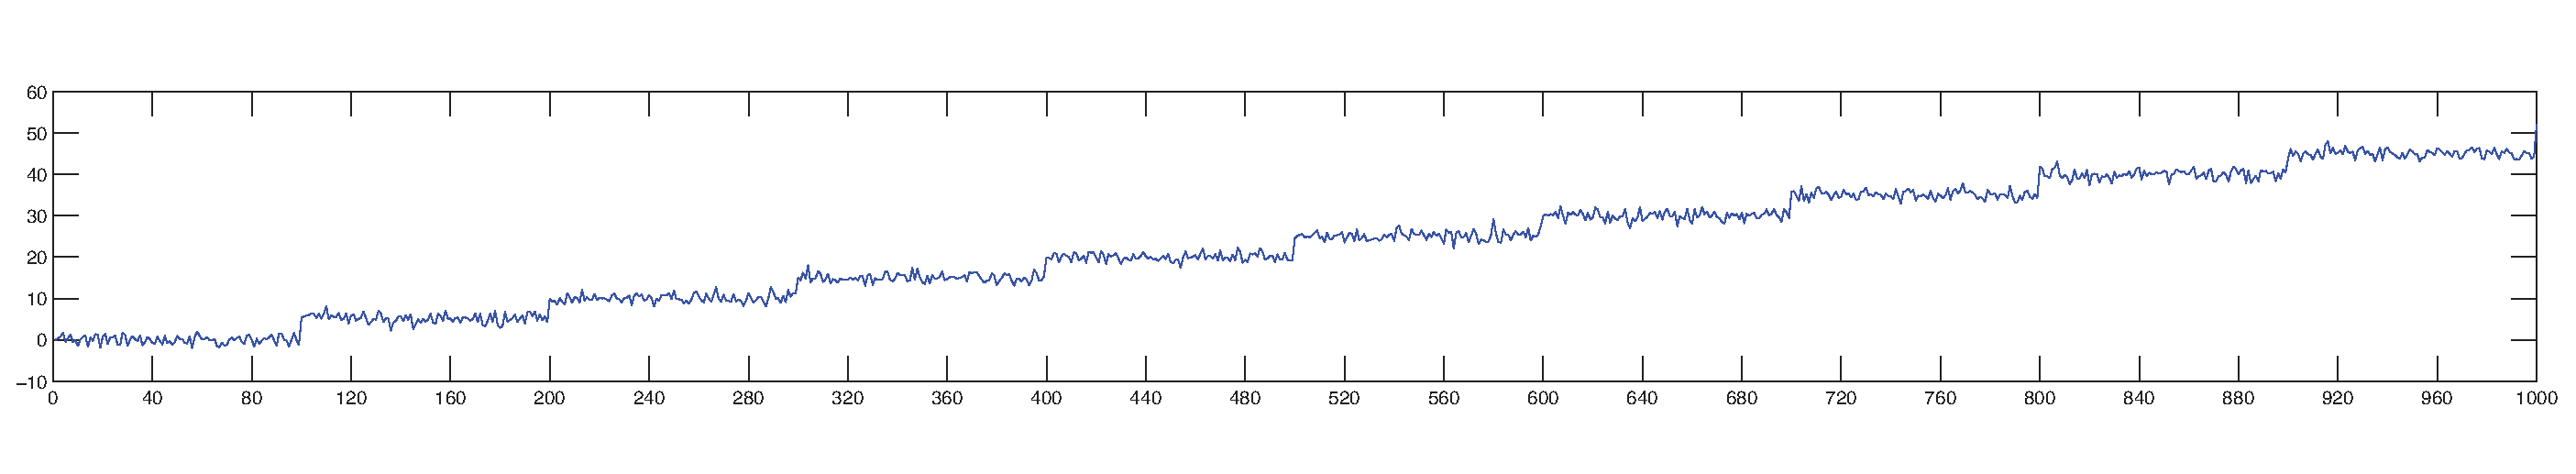
\includegraphics[width=1\textwidth]{./Figures/notes/jumping_mean_camci.eps}
  \caption[Jumping mean camci]{Jumping mean camci}
\end{figure}

\begin{figure}
\centering
  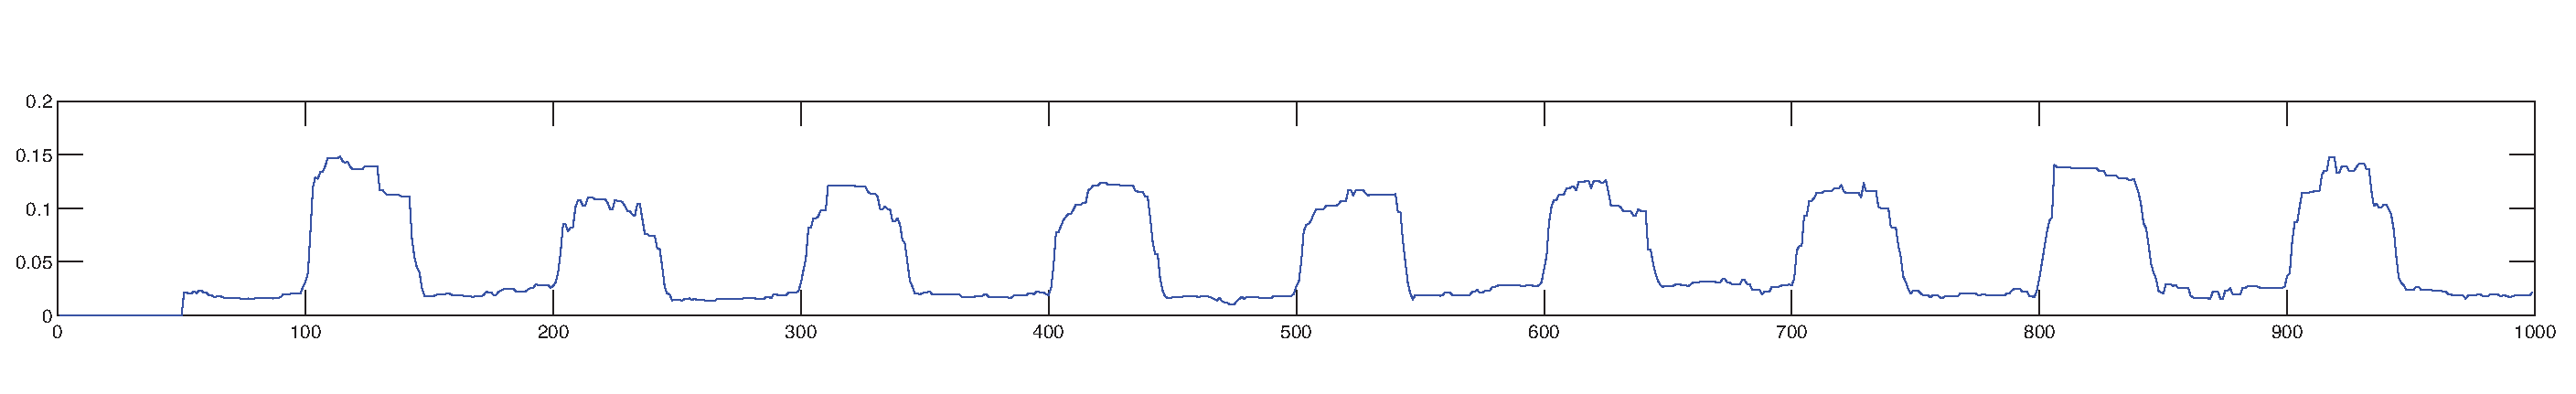
\includegraphics[width=1\textwidth]{./Figures/notes/jumping_mean_camci_thresholds.eps}
  \caption[Jumping mean camci thresholds]{Jumping mean camci, thresholds}
\end{figure}

\begin{figure}
\centering
  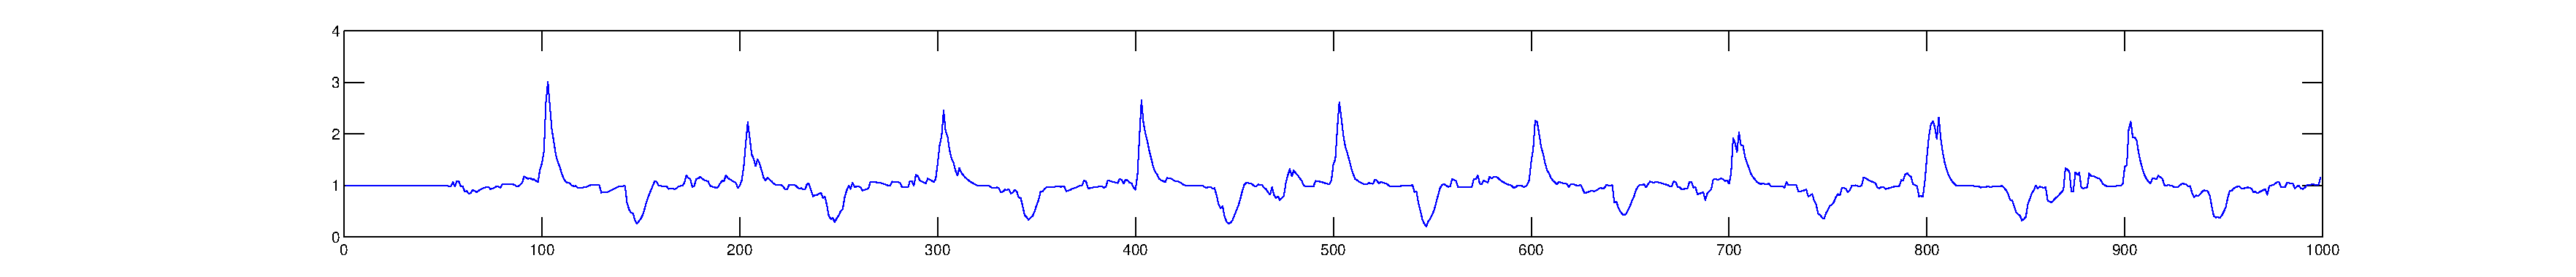
\includegraphics[width=1\textwidth]{./Figures/notes/jumping_mean_camci_ratios_10.eps}
  \caption[Jumping mean camci ratios]{Jumping mean camci ratios, last 10}
  \label{fig:jumping_mean_ratios}
\end{figure}

\begin{figure}
\centering
  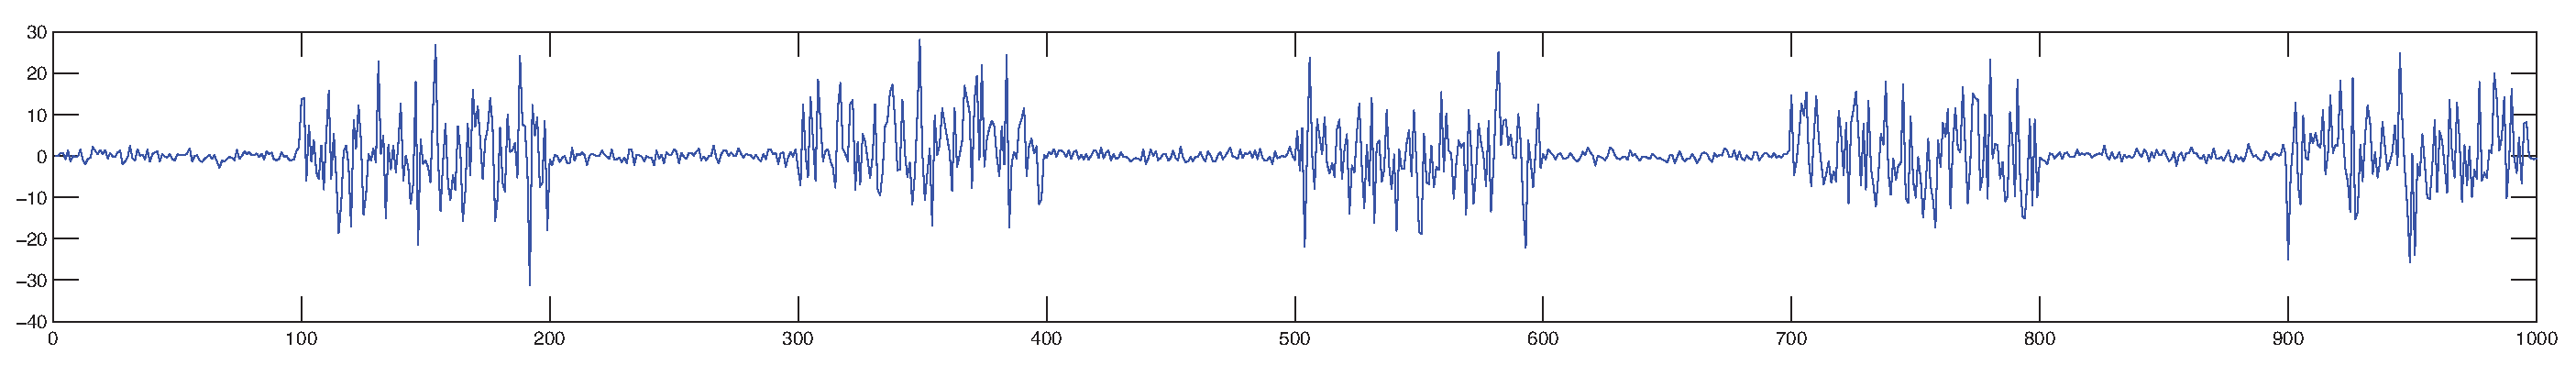
\includegraphics[width=1\textwidth]{./Figures/notes/jumping_variance.eps}
  \caption[Jumping variance]{Jumping variance}
\end{figure}

\begin{figure}
\centering
  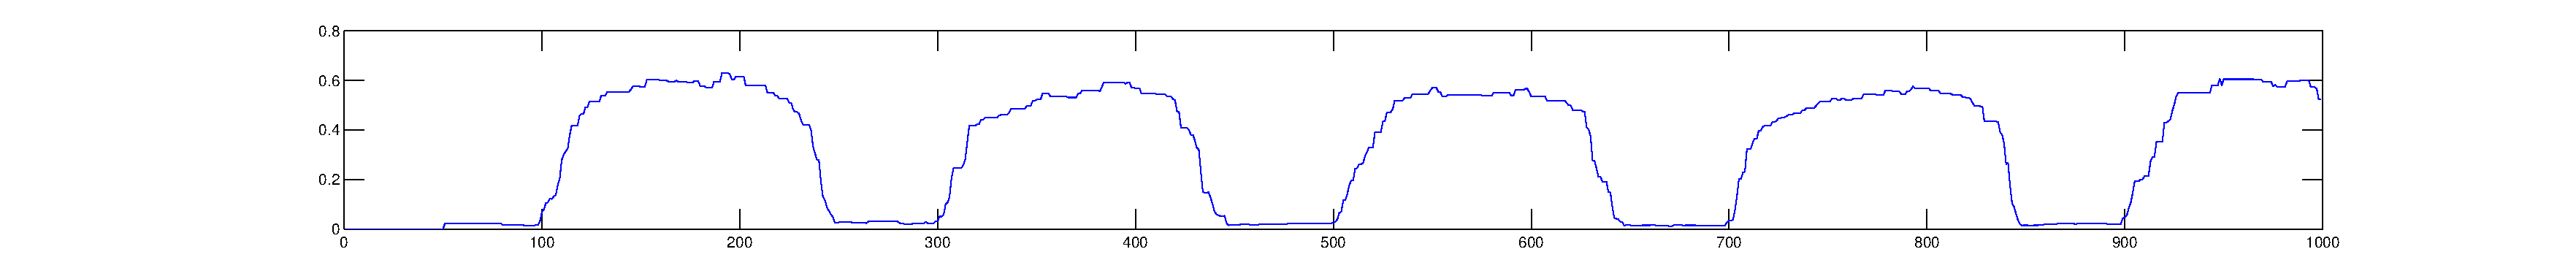
\includegraphics[width=1\textwidth]{./Figures/notes/jumping_variance_thresholds.eps}
  \caption[Jumping variance thresholds]{Jumping variance, thresholds}
\end{figure}

\begin{figure}
\centering
  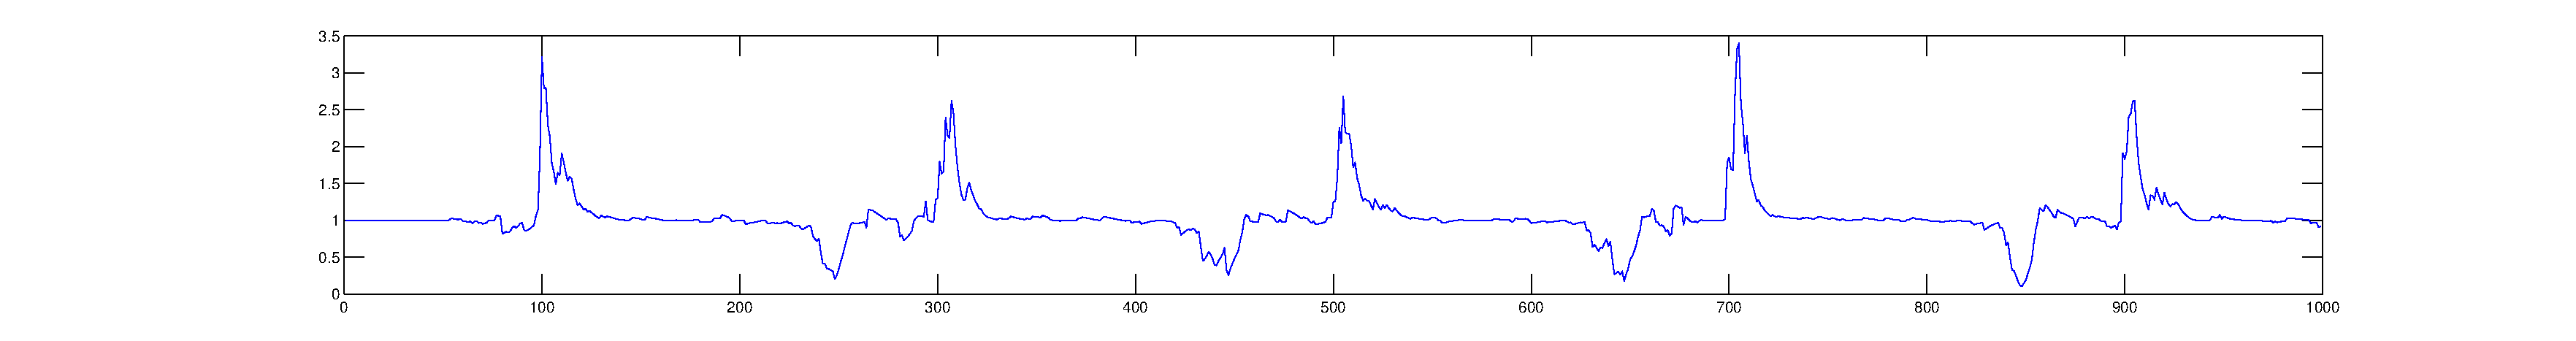
\includegraphics[width=1\textwidth]{./Figures/notes/jumping_variance_ratios_10.eps}
  \caption[Jumping variance ratios]{Jumping variance ratios, last 10}
\end{figure}